\section{Justification}
\label{chp:justification}

Our research group has extensive experience with the Linux ecosystem, including current and past members who have actively contributed to subsystems such as \textit{AMD GPU}, \textit{Industrial I/O (IIO)}, and \textit{Virtual Kernel Mode Setting} (VKMS). Many of these members work professionally as contributors and maintainers, dedicating themselves entirely to Linux development. For instance, our students accounted for 20\% of all accepted contributions to the IIO subsystem during a 90-day period in 2019. Drawing from this experience, our group developed a FLOSS project called \textit{kworkflow} (\textit{kw}), a \textit{Developer Automation Workflow System} (DAWS) designed to streamline and automate workflows for Linux developers.

\textit{kworkflow}\footnote{\href{https://kworkflow.org}{kworkflow site} and \href{https://github.com/kworkflow/kworkflow/}{kworkflow repository}.} provides a unified interface offering solutions to common kernel development challenges, such as abstracting hardware and distribution-specific complexities for tasks like configuring, compiling, and installing custom kernels. It also includes tools for submitting contributions and managing reviews, which have gained traction among industry developers. In 2023, the doctoral student became a maintainer of \textit{kworkflow} and the primary maintainer of its subproject, \textit{patch-hub}\footnote{\href{https://github.com/kworkflow/patch-hub/}{patch-hub repository}.}. This \textit{Terminal User Interface} (TUI), designed for maintainers, simplifies interaction with contributions sent to mailing lists and review management, addressing one of the most critical bottlenecks in the development model.

Our firsthand experience and continuous interaction with researchers and practitioners have generated valuable insights. By systematically mapping Linux kernel development workflows and identifying bottlenecks, we aim to bridge the gap between theory and practice, opening avenues for future research and potentially applying these findings to other software engineering contexts. Pragmatically addressing these bottlenecks with high-quality tools will benefit the Linux ecosystem - contributors, maintainers, testers, and other stakeholders - by streamlining complex processes, enhancing productivity, reducing workload, increasing contribution throughput, and scaling the workforce. Ensuring these tools are FLOSS is crucial, as it allows the Linux community to provide feedback and contribute organically, aligning with \textbf{Objective 2}.

Additionally, addressing these challenges could free up resources to tackle underprioritized issues, such as the project environmental sustainability. Given Linux pervasive role in technology - from embedded systems and Internet infrastructure to supercomputers and AI machine learning model training - making it more environmentally friendly could have a significant global impact. Furthermore, improving Linux quality as a software solution could create a positive ripple effect across modern computing, reinforcing its importance as a cornerstone of FLOSS development.

\subsection{Evidence about the gap in academic understandings of the Linux kernel development model}

A symptom of the misleading conclusions from the scientific community about the Linux kernel development model is the divergent definitions given by different authors.

For \textit{Rigby et al. (2014)}~\cite{rigby2014-peer-review}, the model is a dictatorship that relegates newcomers and has a rigid and subservient culture; For \textit{Fogel (2017)}~\cite{fogel2017-producing-oss}, the ``forkability'' of the project results in a ``benevolent dictator'' model where Linus does not have full authority on the project; \textit{Lindberg et al. (2014)}~\cite{lindberg2014-theorizing}, believes that a core group of developers takes most of the reviews and is also exclusively responsible for approving code changes, following a \textit{Cathedral model}~\cite{raymond1999-cathedral}; finally, \textit{Shaikh and Henfridsson (2017)}~\cite{shaikh2017-governing-oss} argue that four governance types coexist in the Linux kernel development: autocracy, oligarchy, federation, meritocracy.

The lack of a consensus on a primordial aspect, such as categorizing the Linux kernel development model, indicates how academic investigations are at an early stage. At last, \textit{Wen (2021)}~\cite{wen2021-masterthesis}, using the qualitative research method of \textit{Directed Content Analysis}, produced mind maps that describe the Linux kernel development model. They showed, at large, gaps and misconceptions from the scientific community when crossed with community perspectives. 

\subsection{Empirical evidence about the unsustainability of the Linux kernel development model}

We have produced empirical quantitative evidence indicating that the Linux kernel development model may be unsustainable due to its current structure\footnote{These experiments are reproducible with \textit{Docker} following the instructions in \href{https://github.com/davidbtadokoro/phd-experiments/tree/master/linux-stats}{this repository}.}. Figures \ref{fig:loc-linux}, \ref{fig:maintainers-linux}, and \ref{fig:commits-linux} are plots that show statistics about the development of Linux over the last 10 years. Due to the periodicity of releases that follow subsequent six to eight-week cycles, we can use the Linux versions as consistent timestamps to analyze the evolution of the project. In this sense, the aforementioned figures have the Linux versions in the abscissa from 3.19 (launched on 8 February 2015) until 6.13 (launched on 20 January 2025).

\begin{figure}[h!]
    \centering
    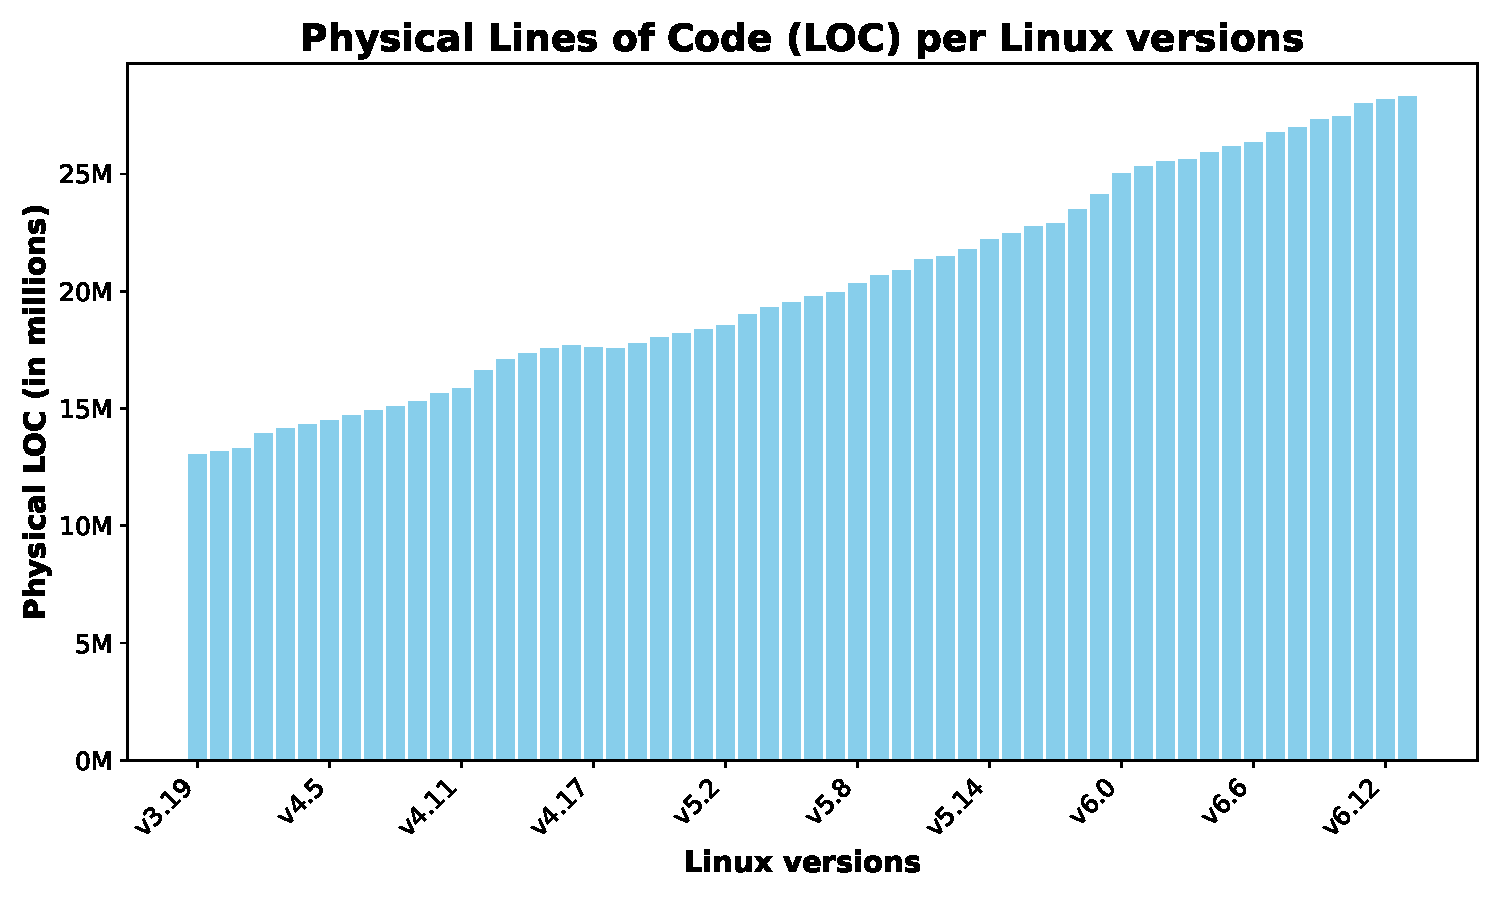
\includegraphics[width=0.75\textwidth]{images/phys-loc.pdf}
    \caption{Linux physical LOC from version 3.19 to 6.13.\label{fig:loc-linux}}
\end{figure}

\begin{figure}[h!]
    \centering
    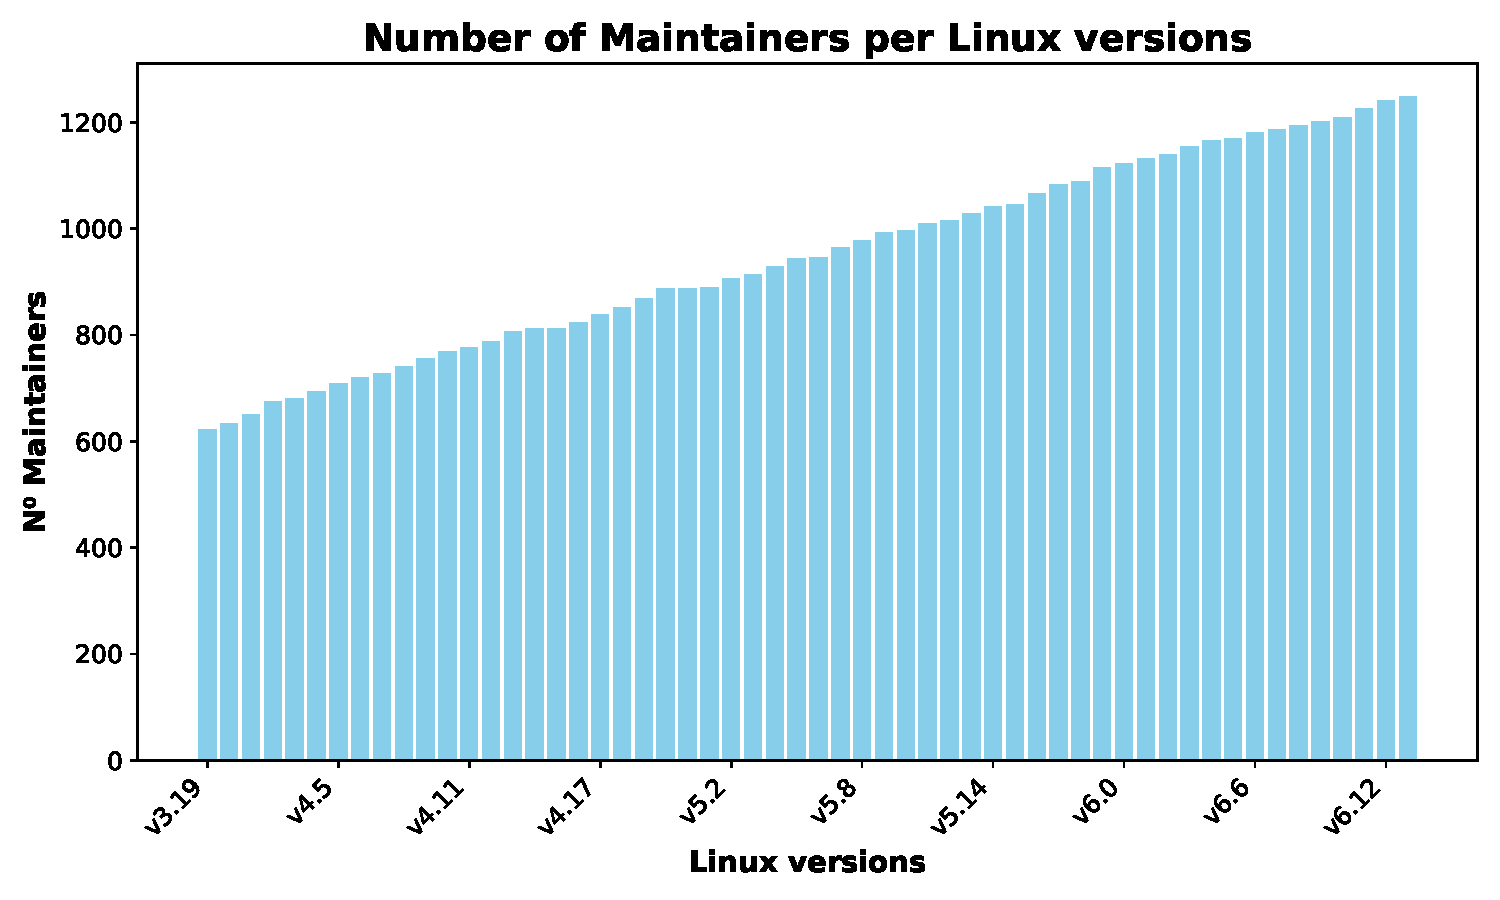
\includegraphics[width=0.75\textwidth]{images/maintainers.pdf}
    \caption{Number of Linux maintainers from version 3.19 to 6.13.\label{fig:maintainers-linux}}
\end{figure}

\begin{figure}[h!]
    \centering
    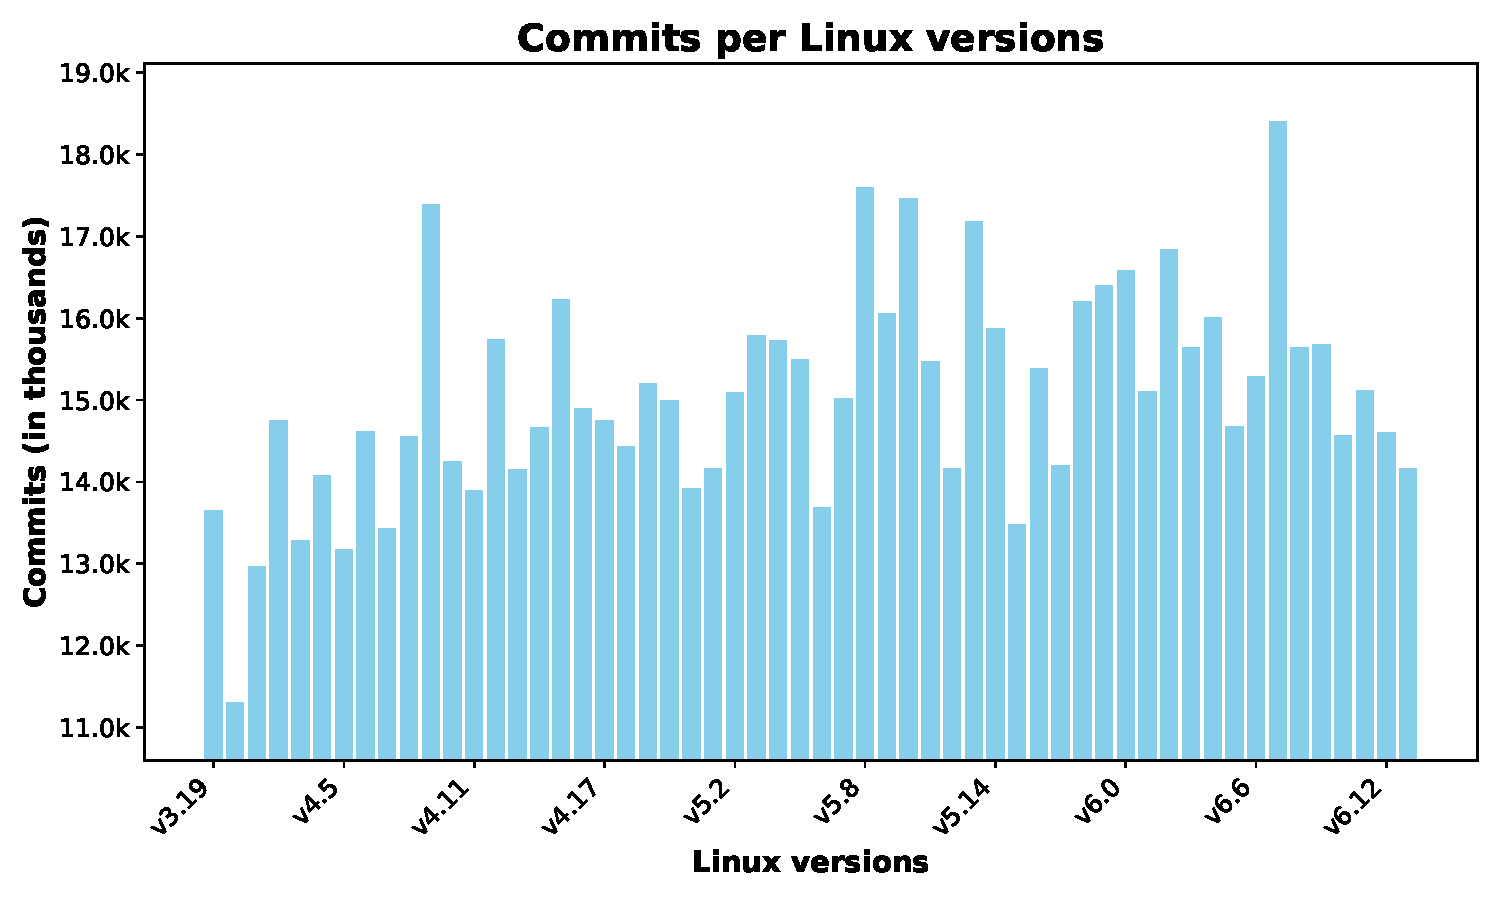
\includegraphics[width=0.75\textwidth]{images/commits.pdf}
    \caption{Commits in the development cycle of versions 3.19 to 6.13.\label{fig:commits-linux}}
\end{figure}


Figure \ref{fig:loc-linux} displays the increase of \textit{physical Lines of Code} (physical LOC)\footnote{A software metric that measures the number of source lines of code (excluding blank ones and comments) in a program source code.} and shows how the Linux kernel codebase is steadily growing regarding its size. We can derive that the project complexity is also growing as more features, drivers, and the like are continuously being merged. Interestingly, by investigating the entries in the \texttt{MAINTAINERS} file, we produced Figure \ref{fig:maintainers-linux} that depicts how the number of maintainers steadily increases.

Notwithstanding the increase in the number of maintainers, we can see in Figure \ref{fig:commits-linux} that the amount of commits in each development cycle of Linux fluctuates between 13000 and 17500 since version 3.19, excluding outliers. Every commit is different as an individual commit can be a massive change, while a set of ten commits can be a single line change ten times, and a difference of four and a half thousand commits is expressive, so we can not derive solid conclusions based on these statistics. However, just the fact that the number of commits has fluctuated consistently indicates that the contribution throughput does not scale in the same fashion as the number of maintainers.

The Linux kernel development model functions as a self-sustaining and highly specialized ecosystem. However, by extrapolating the empirical evidence, we can assume that the model reliance on a continuous influx of skilled contributors, a highly dedicated pool of maintainers, and ever-increasing code complexity suggests characteristics similar to an ``economic bubble'' where short-term growth may mask long-term sustainability risks.
